\subsubsection{V-Cycle Scheme}\label{subsubsection: V-Cycle Scheme}

\textbf{\underline{Purpose}}. The V-Cycle Scheme has the powerful \textbf{ability to move between fine and coarse grids} in a \emph{structured manner}, \emph{efficiently} and \emph{recursively} \textbf{reducing errors at all levels}. It is very similar to the Two-Grid scheme, but the V-Cycle version allows us to go as deep as we want (or can). The general idea is:
\begin{enumerate}
    \item Given an initial guess $\mathbf{x}_{h}^{\left(0\right)}$;
    \item While the stopping criteria is met:
        \begin{enumerate}
            \item Compute:
            \begin{equation}
                \mathbf{x}_{h}^{\left(k+1\right)} = \mathrm{MG}\left(\mathbf{x}_{h}^{\left(k\right)}, \mathbf{b}_{h}, \nu_{1}, \nu_{2}, J\right)
            \end{equation}
        \end{enumerate} 
\end{enumerate}
As in the Two-Grid scheme, the arguments are the same, but the difference is the parameter $J$, which indicates the maximum depth of the algorithm. However, when the $\mathrm{MG}$ method is invoked, the algorithm is executed:
\begin{enumerate}
    \item\label{enumerate: v-cycle scheme - Fine Grid Smoothing (pre-smoothing)} \textbf{Fine Grid Smoothing (pre-smoothing)}. We start at the finest grid level (top of the V shape). We apply $\nu_{1}$ iterations of a smoothing algorithm such as Jacobi, on the system $A_{h}\mathbf{x}_{h} = \mathbf{b}_{h}$ with the initial guess $\mathbf{x}_{h}^{\left(k\right)}$ to reduce high-frequency errors. The solution that we obtain is $\mathbf{y}_{h}^{\left(\nu_{1}\right)}$.
    \begin{equation*}
        \mathbf{y}_{h}^{\left(\nu_{1}\right)} \leftarrow \text{Relax } \nu_{1} \text{ times on } A_{h}\mathbf{x}_{h} = \mathbf{b}_{h}
    \end{equation*}

    \item \textbf{Compute Fine Grid Residual}. Calculate the residual on the fine grid $\mathbf{r}_{h}^{\left(\nu_{1}\right)} = \mathbf{b}_{h} - A_{h}\mathbf{y}_{h}^{\left(\nu_{1}\right)}$:
    \begin{equation*}
        \mathbf{r}_{h}^{\left(\nu_{1}\right)} \leftarrow \mathbf{b}_{h} - A_{h}\mathbf{y}_{h}^{\left(\nu_{1}\right)}
    \end{equation*}

    \item\label{enumerate: v-cycle scheme - Restriction to Coarse Grid} \textbf{Restriction to Coarse Grid}. Move the residual $\mathbf{r}_{h}^{\left(\nu_{1}\right)}$ from the fine grid to the coarse grid to obtain the residual $\mathbf{r}_{2h}^{\left(\nu_{1}\right)} = I_{h}^{2h} \mathbf{r}_{h}^{\left(\nu_{1}\right)}$:
    \begin{equation*}
        \mathbf{r}_{2h}^{\left(\nu_{1}\right)} = I_{h}^{2h} \mathbf{r}_{h}^{\left(\nu_{1}\right)}
    \end{equation*}

    \item \textbf{Recursive V-Cycle on Coarser Grid}. Check if the coarsest level is the desired one, in other words, if we are at the coarsest level we requested when we first invoked the algorithm.

    If the level is the maximum depth requested ($j = $ actual coarsest level), solve the problem or find an approximate solution using direct methods. If we are at this level, we are at the bottom of the V-shape. Otherwise, if the level is not the desired one, we apply the V-cycle process recursively on the coarsest grid, repeating steps \ref{enumerate: v-cycle scheme - Fine Grid Smoothing (pre-smoothing)} through \ref{enumerate: v-cycle scheme - Restriction to Coarse Grid} on progressively coarser grids until the coarsest grid is reached.
    \begin{equation*}
        \begin{cases}
            \text{Solve } A_{2h}\mathbf{e}_{2h} = \mathbf{r}_{2h}^{\left(\nu_{1}\right)} & \text{if } J = \text{ actual coarsest level} \vspace{.8em}\\
            \mathbf{e}_{2h} = \mathrm{MG}\left(\mathbf{0}, \mathbf{r}_{2h}^{\left(\nu_{1}\right)}, \nu_{1}, \nu_{2}, j-1\right) & \text{otherwise}
        \end{cases}
    \end{equation*}

    \item\label{enumerate: v-cycle scheme - Interpolate back to Fine Grid} \textbf{Interpolate back to Fine Grid}. If we are here, the recursion has reached the maximum depth. Now we have to come back to the surface and follow the right side of the V-shape. Therefore, we transfer the correction $\mathbf{e}_{2h}$ calculated in the previous step from the coarse to the fine grid using an interpolation operator $I_{2h}^{h}$ (page \pageref{subsubsection: Interpolation Operator}):
    \begin{equation*}
        \mathbf{e}_{h} = I_{2h}^{h} \mathbf{e}_{2h}
    \end{equation*}

    \item \textbf{Update and apply correction}. Correct the approximation obtained on the fine grid with the error estimate obtained on the coarse grid. Applying this correction refines the solution on the fine grid, reducing the overall error:
    \begin{equation*}
        \mathbf{y}_{h}^{\left(\nu_{1}+1\right)} \leftarrow \mathbf{y}_{h}^{\left(\nu_{1}\right)} + \mathbf{e}_{h}
    \end{equation*}

    \item \textbf{Fine Grid Smoothing (post-smoothing)}. Do $\nu_{2}$ iterations using a chosen smoother (e.g. Jacobi) on the system $A_{h}\mathbf{x}_{h} = \mathbf{b}_{h}$ starting with the updated solution (initial guess) $\mathbf{y}_{h}^{\left(\nu_{1}+1\right)}$. The solution after these iterations is $\mathbf{y}_{h}^{\left(\nu_{1}+1+\nu_{2}\right)}$.
    
    These additional smoothing iterations are essential to refine the solution and ensure that both high and low frequency errors are adequately addressed. It can also help stabilize the solution by ensuring that any residual errors are minimized.
    \begin{equation*}
        \mathbf{y}_{h}^{\left(\nu_{1} + 1 + \nu_{2}\right)} \leftarrow \text{Relax } \nu_{2} \text{ times on } A_{h}\mathbf{x}_{h} = \mathbf{b}_{h}
    \end{equation*}

    \item\label{enumerate: v-cycle scheme - Recursively return to the surface} \textbf{Recursively return to the surface}. We return the result obtained in the previous step $\mathbf{y}_{h}^{\left(\nu_{1} + 1 + \nu_{2}\right)}$ at the previous level of coarsest. Since we are in a recursive path, if the previous caller is the main, then the method stops, otherwise the previous caller recalculates its results from step \ref{enumerate: v-cycle scheme - Interpolate back to Fine Grid} to \ref{enumerate: v-cycle scheme - Recursively return to the surface}, and so on.
    \begin{equation*}
        \mathbf{x}_{h}^{\left(k+1\right)} \leftarrow \left(j-1 \text{ recursive steps}\right) \leftarrow \mathbf{y}_{h}^{\nu_{1} + 1 + \nu_{2}}
    \end{equation*}
\end{enumerate}
Note that the algorithm seems very similar to the Two-Grid Scheme because the V-Cycle Scheme is an extension applied $j$ times! In Figure \ref{fig: V-Cycle Scheme}, we can see why the V-cycle scheme has a V-shape.

\highspace
However, the V-cycle scheme is only one of several MG cycling schemes. Other types of schemes are W-cycle and F-cycle, and can be analyzed at the following MIT \href{https://math.mit.edu/classes/18.086/2006/am63.pdf}{link}.

\newpage

\begin{figure}[!htp]
    \centering
    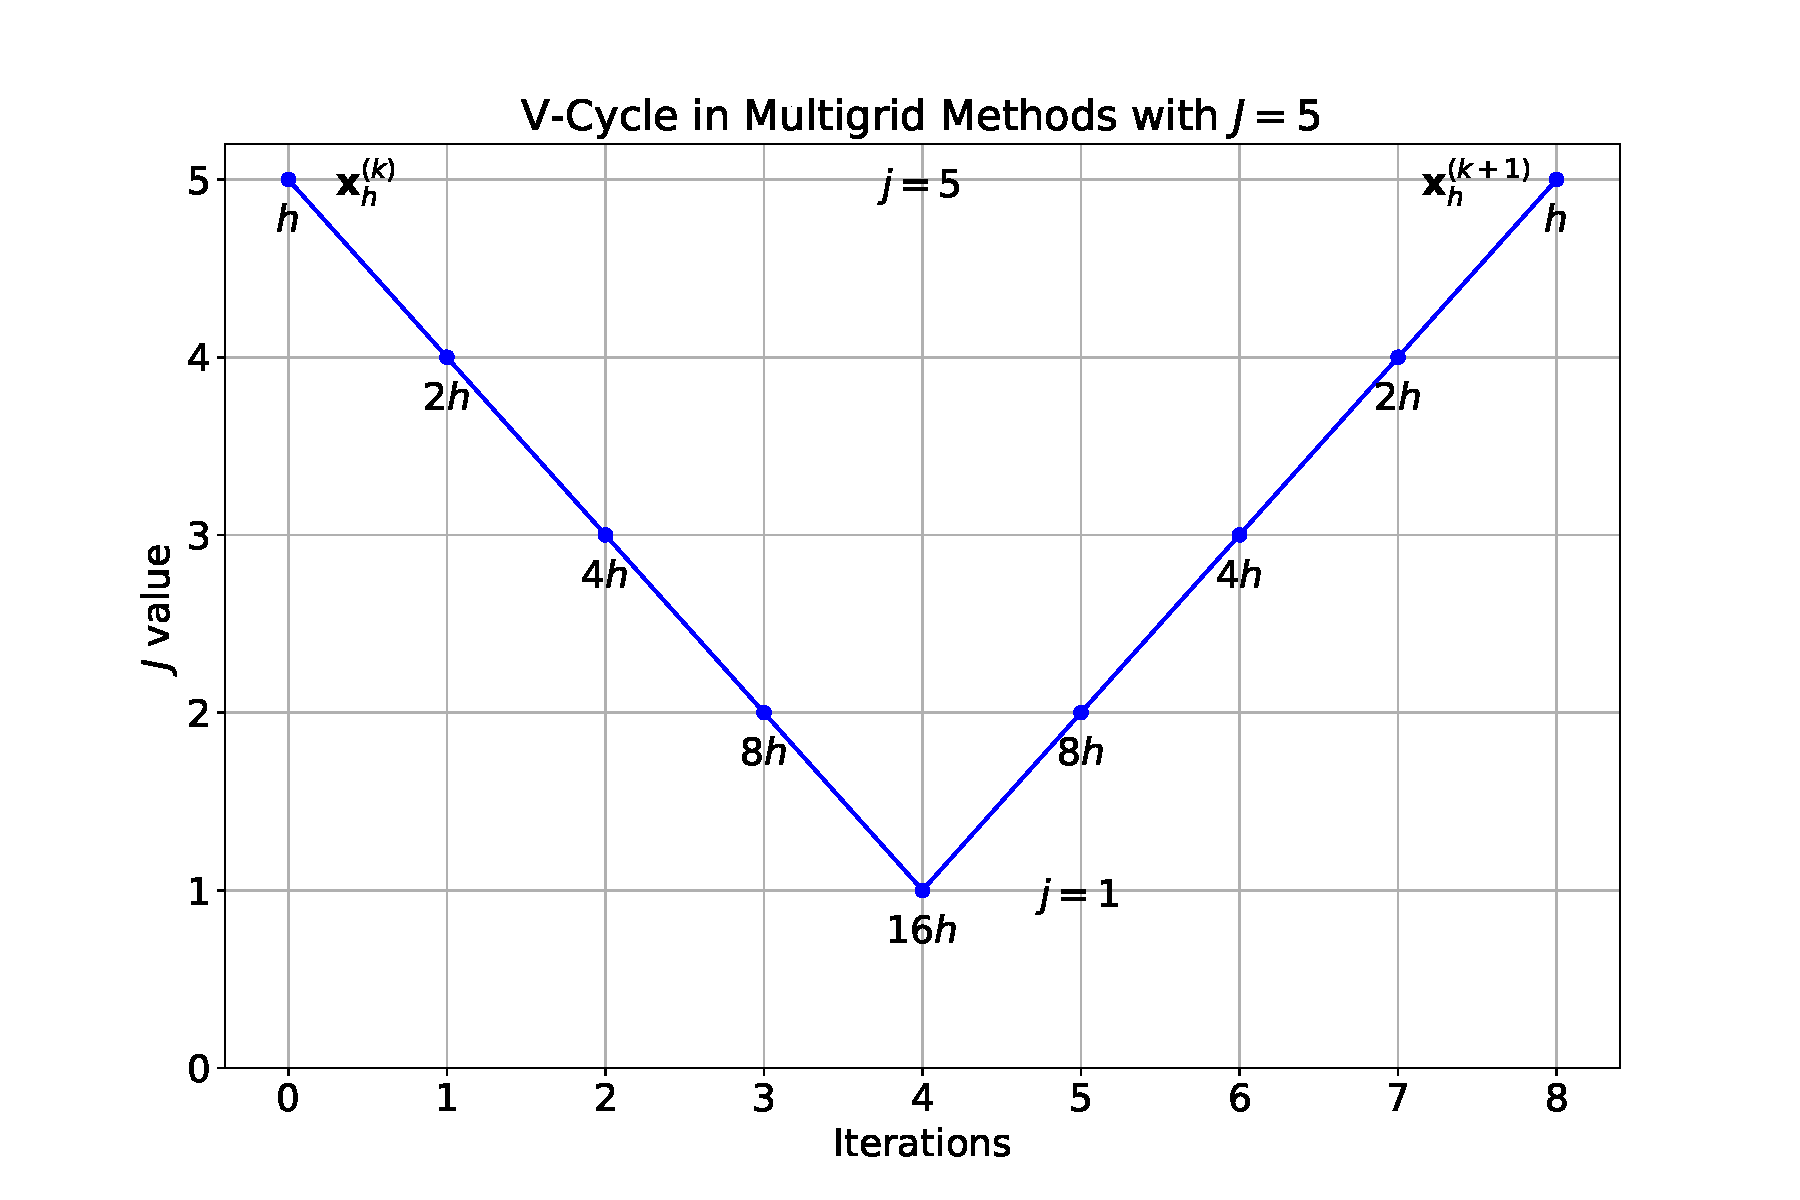
\includegraphics[width=\textwidth]{img/v-cycle-scheme.pdf}
    \caption{V-Cycle Scheme.}
    \label{fig: V-Cycle Scheme}
\end{figure}

\begin{flushleft}
    \textcolor{Red2}{\faIcon{dollar-sign} \textbf{How much does it cost?}}
\end{flushleft}
The V-Cycle Scheme has a \textbf{convergence less than one and independent} of $h$ and \textbf{it costs only} $O\left(n^{d} \log\left(n\right)\right)$.

\highspace
At each level $j$ the values $\mathbf{x}_{h}^{\left(k\right)}$ and $\mathbf{b}_{h}$ must be stored. Also, each successively coarser grid requires progressively less memory because the number of grid points is reduced by a factor at each level. In $d$ dimensions, the coarse grid has $\approx 2^{-d}$ the number of points as the finer grid. Therefore the memory requirement is:
\begin{equation*}
    \text{Storage cost } \approx \dfrac{2n^{d}}{1 - 2^{-d}}
\end{equation*}
Furthermore, for $d = 1$ the memory requirement is less than twice that of the fine-grid problem alone.